\documentclass[10pt,a4paper,onecolumn]{article}

% packages
\usepackage[a4paper, margin=3cm]{geometry}
\usepackage[utf8]{inputenc}
\usepackage[english]{babel}

\usepackage{graphicx}
\usepackage{xcolor}
\usepackage{import}

\usepackage{amsmath}
\usepackage{amsfonts}
\usepackage{amssymb}
\usepackage{amsthm}

\usepackage{hyperref}
\usepackage[noabbrev]{cleveref}
\usepackage{autobreak}

% paragraph spacing
\setlength{\parindent}{0em}
\setlength{\parskip}{1em}

% define vector and matrix representations
%\renewcommand{\vec}[1]{\textbf{#1}}
\renewcommand{\vec}[1]{\underline{#1}}
%\renewcommand{\vec}[1]{\uppercase{#1}}
\newcommand{\mat}[1]{#1}

% set graphics path
\graphicspath{{images/}}

% Authors and Affiliations
\title{Equations}
\author{Maximilian Gruber}    % maximilian.gruber@ptb.de
\date{November 2020}
    
\begin{document}
    \maketitle
    We consider sensors with linear affine input-output behavior. The real transfer model with parameters $(\alpha_j, \beta_j)$ are unknown. From a calibration the estimated compensation model is known and given by parameters $(a_j, b_j)$ of another affine linear model. The inverse of the compensation model is the estimated transfer model. 
    \begin{figure}[h]
        \centering
        %\def\svgwidth{0.9\linewidth}
        %\input{images\....pdf_tex}
        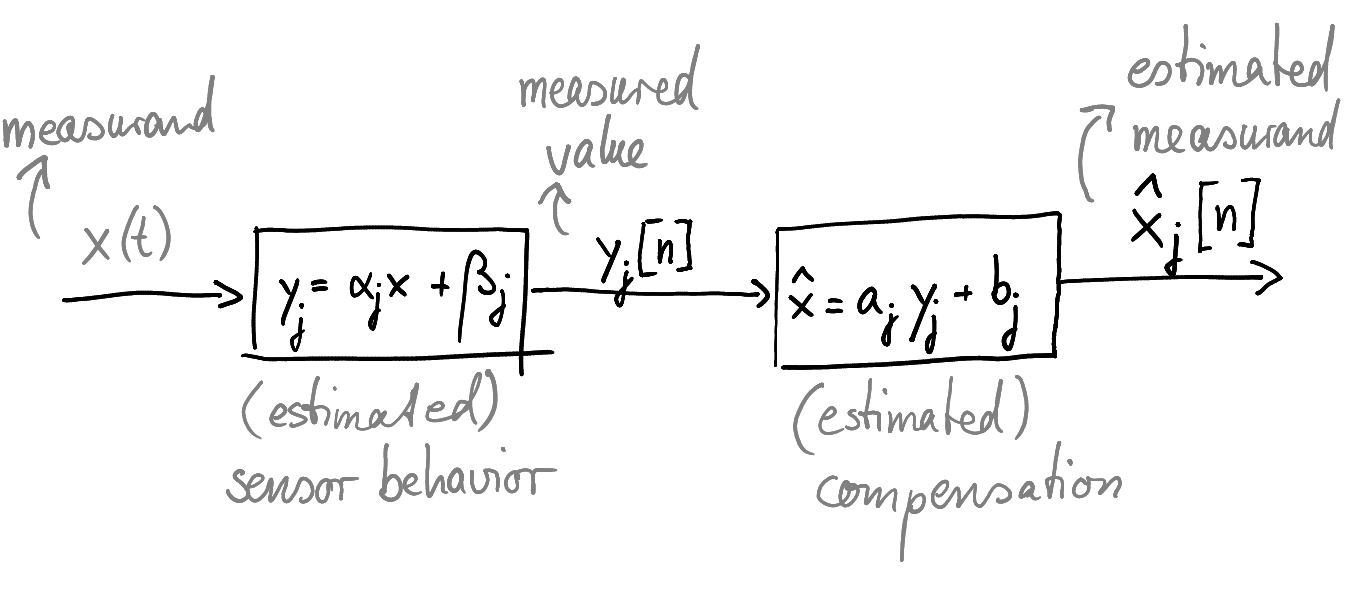
\includegraphics[width=0.9\linewidth]{system_description.png}
        \caption{Assumed system structure for estimation}
        \label{fig:filterbank}
    \end{figure}
    
    \section{The Stankovic algorithm}
    The scalar input signal $x(t)$ ((bounded) stochastic stationary process) is measured by a network $\mathcal{N}$ of sensors. The $i$-th sensor measures $y_j(t) = \alpha_j * x(t) + \beta_j$. To estimate the original input, the inverse model $\hat{x}_j = a_j * y_j(t) + b_j$ is required. 
    
    For new a sensor $i$ the parameters $(a_i, b_i)$ are unknown and can be estimated from the neighbors $\mathcal{N}_i$ of the new sensor. This can be achieved by the proposed update equation from [stankovic\_2018], which is based on a gradient optimization scheme:
    \begin{align}
        \vec{\theta}[n+1] &= \vec{\theta}[n] + \delta(t) * \vec{\nabla} J
    \end{align}
    With
    \begin{align}
        \vec{\theta} &= [ a_i, b_i ]^T \\
        \vec{\nabla} J &=  \sum_{j \in \mathcal{N}_i} \gamma_{ij} \mathbb{E}\left\{ ( \hat{x}_j[n] - \hat{x}_i[n]) *
            \begin{bmatrix} y_i[n-d] \\ 1 \end{bmatrix} \right\} \nonumber \\
        &= \sum_{j \in \mathcal{N}_i} \gamma_{ij} \begin{bmatrix} - a_i[n]*{y_i[n-d]}^2 + (\hat{x}_j[n] - b_i[n]) * y_i[n-d]\\ - a_i[n]*y_i[n-d] + (\hat{x}_j[n] - b_i[n]) \end{bmatrix}
    \end{align}
    
    \section{Uncertainty of the Parameter Update}
    \begin{align}
        \vec{\theta}[n+1] &= f(a_i[n], b_i[n], y_i[n-d], \underbrace{\hat{x}_j[n], \dots}_{j \in \mathcal{N}_i}) \\
        U_{\vec{\theta}[n+1]} &= C * U * C^T
    \end{align}
    
    With covariance of the inputs $U$ and sensitivities $C$. Note that $U$ contains information from $U_{\vec{\theta}[n]}$ and $\delta(t)$ is assumed to be deterministic (e.g. constant). 
    \begin{align}
        U &= 
        \begin{bmatrix}
            u(a_i[n])^2 & u(a_i[n], b_i[n])) & 0 & 0 & \\
            u(a_i[n], b_i[n]) & u(b_i[n]))^2 & 0 & 0 & \cdots \\
            0 & 0 & u(y_i[n-d])^2 & 0 & \\
            0 & 0 & 0 & u(\hat{x}_j[n])^2 & \\
            & \vdots & & & \ddots
        \end{bmatrix} \\
        C &=
        \begin{bmatrix}
            \frac{\partial a_i[n+1]}{\partial a_i[n]} & \frac{\partial a_i[n+1]}{\partial b_i[n]} & \frac{\partial a_i[n+1]}{\partial y_i[n]} & \frac{\partial a_i[n+1]}{\partial \hat{x}_j[n]} \\
            \frac{\partial b_i[n+1]}{\partial a_i[n]} & \frac{\partial b_i[n+1]}{\partial b_i[n]} & \frac{\partial b_i[n+1]}{\partial y_i[n]} & \frac{\partial b_i[n+1]}{\partial \hat{x}_j[n]} \\
        \end{bmatrix}
    \end{align}
    
    And:
    \begin{align}
        \frac{\partial a_i[n+1]}{\partial a_i[n]} &= 1 + \delta(t) * \sum_{j \in \mathcal{N}_i} \gamma_{ij} * (- {y_i}[n-d]^2) \\
        \frac{\partial a_i[n+1]}{\partial b_i[n]} &= 0 + \delta(t) * \sum_{j \in \mathcal{N}_i} \gamma_{ij} * (- y_i[n-d]) \\
        \frac{\partial a_i[n+1]}{\partial y_i[n]} &= 0 + \delta(t) * \sum_{j \in \mathcal{N}_i} \gamma_{ij} * (-2 a_i[n] * y_i[n-d] + \hat{x}_j[n] - b_i[n]) \\
        \frac{\partial a_i[n+1]}{\partial \hat{x}_j[n]} &= 0 + \delta(t) * \gamma_{ij} * y_i[n-d]\\
        \nonumber\\
        \frac{\partial b_i[n+1]}{\partial a_i[n]} &= 0 + \delta(t) * \sum_{j \in \mathcal{N}_i} \gamma_{ij} * (- y_i[n-d]) \\
        \frac{\partial b_i[n+1]}{\partial b_i[n]} &= 1 + \delta(t) * \sum_{j \in \mathcal{N}_i} \gamma_{ij} * (- 1) \\
        \frac{\partial b_i[n+1]}{\partial y_i[n]} &= 0 + \delta(t) * \sum_{j \in \mathcal{N}_i} \gamma_{ij} * (- a_i[n]) \\
        \frac{\partial b_i[n+1]}{\partial \hat{x}_j[n]} &= 0 + \delta(t) * \gamma_{ij}
    \end{align}
    
    
    
    
    \section{Uncertainty of Output of linear affine Transfer-Function}
    
    \section{Uncertainty of the estimated inverse Model-Parameters}
    
\end{document}